\hypertarget{a-cidade-brasileira-do-suxe9culo-xix-e-a-construuxe7uxe3o-de-discursos-nacionais}{%
\section{A cidade brasileira do século XIX e a construção de discursos
nacionais}\label{a-cidade-brasileira-do-suxe9culo-xix-e-a-construuxe7uxe3o-de-discursos-nacionais}}

A construção de um discurso sobre o caráter moral e histórico da nação,
no século XIX, implica distinguir os aspectos peculiares na geografia,
nos costumes e na organização política de uma sociedade. É o que faz,
por exemplo, o pintor Jean-Baptiste Debret (1768--1848), um dos
protagonistas da Missão francesa que tanta polêmica suscitará mais
adiante, ao propor como objeto da sua publicação \emph{Voyage
pittoresque et historique au Brésil} os ``pontos característicos dos
objetos circundantes'' para assim constituir uma ``obra histórica''
\autocite[p.~i--ii]{debret:1834voyage1}. Para tanto, Debret atribui
papel preponderante ao seu ofício --- o desenho ---, mas não prescinde
de textos explicativos, especialmente necessários para tornar as cenas
do cotidiano escravista compreensíveis para o público francês.

Representar a aparência visível da cidade, especialmente com o reforço
da cena anedótica ou da curiosidade repulsiva, cumpre então seu papel de
instrumento privilegiado para caracterizar a fisionomia, por assim
dizer, do corpo social. Assim fazendo, Debret insere-se numa tradição de
arte metafórica, extraída da literatura no século XVII
\autocite{delft:1993nature}, codificada por Charles Le Brun
\autocite{dabbs:2002characterising65} e introduzida no domínio da
arquitetura e do desenho urbano com o neoclassicismo ``visionário'' da
idade do Iluminismo \autocite{pigafetta:2009passioni}. A
\emph{caracteriologia} classicista se constitui, assim, sobre a visão de
mundo cartesiana de uma natureza --- inclusive humana --- imutável,
arcabouço sobre o qual erigem-se as particularidades nacionais e
individuais.

Na hierarquia acadêmica dos gêneros pictóricos, os temas religiosos e
mitológicos --- estes compreendendo também a história antiga --- são
aptos a expressarem os caracteres tidos como universais. À história
moderna, por sua vez, correspondem os caracteres nacionais. Estes
gêneros ocupam o patamar superior, predominantemente preenchido pela
encomenda da Igreja, do Estado, ou dos agentes privados da elite
política.

No entanto, em contraste com as academias europeias, defensoras da
hierarquia dos gêneros de pintura, o contexto artístico brasileiro no
século XIX é de predomínio da pintura de gênero e, secundariamente, da
paisagem \autocite{squeff:2012galeria}. Esses dois domínios se confundem
na representação de cenas urbanas, que gozam, no Brasil, de papel
informativo e estético peculiar. Como uma espécie de \emph{exotismo para
dentro}, essas obras, expostas nos Salões de Belas Artes ou compondo
coleções particulares, tecem um discurso político e etnográfico sobre a
cidade real vivenciada pelo artista e a civilização urbana por ele
imaginada. A literatura do início do século XX, programaticamente
comprometida com um projeto de modernização cultural, tem relativo
sucesso em relegar essa figuração da civilização oitocentista ao papel
de modorrento retrato do atraso nacional
\autocite{bernd:1992literatura}.

\begin{center}\rule{0.5\linewidth}{0.5pt}\end{center}

A não centralidade do fato urbano na construção de discursos formativos
da nacionalidade brasileira, ao longo do século XIX, é evidenciada,
acima de tudo, na abstração indianista da literatura nacional. Como
lembra Zilá Bernd, a imagem do ``autóctone como antepassado mítico''
está atrelada a uma celebração sacralizada da natureza intocada ---
posto que o índio é parte dela, ao contrário do engenhoso português
\autocite[p.~37--38]{bernd:1992literatura}. Invisível desde o Rio de
Janeiro, cujos círculos literários são os produtores privilegiados dos
discursos sobre a nacionalidade, e combatida por missionários e
militares nas fronteiras demográficas do País, a espacialidade indígena
permanece ausente enquanto o índio idealizado faz furor na literatura da
segunda metade do século.

A mitológica harmonia do Romantismo entre português e indígena é
transposta para o Naturalismo do final do século, escancarando-se ao
mesmo tempo a exclusão do componente negro na formação étnica e cultural
brasileira, relegado por Euclides da Cunha a estrato racial e cultural
inferior ao do sertanejo mestiço de branco e índio
\autocite[p.~44]{bernd:1992literatura}, assim como reafirmando a
exclusividade luso-brasileira na produção do território.

De fato, o ordenamento jurídico construído ao longo do século XIX, em
especial pela Lei de Terras, não apenas reafirma a estratificação social
e racial na estrutura fundiária do País, como também restringe a
possível contribuição do imigrante ao processo de urbanização e ocupação
do território, colocando-a sempre sob a égide do Estado e dos grandes
proprietários já estabelecidos \autocite[p.~198]{depaula:2011processo}.

Se os textos críticos ou históricos na primeira metade do século XIX dão
pouco ou nenhum lugar à cidade e à urbanização, as representações
visuais do mesmo período compõem um acervo muito mais informativo. Desde
o período vice-real, afirma-se uma cultura visual secular que dá ao
primeiro discípulo brasileiro de Debret, Manuel de Araújo Porto Alegre
(1806--1879) ensejo para ver aí o primeiro ``impulso do espírito
nacional'' nas artes \autocite[p.~50]{magalhaes:1834resume}. Neste
contexto, destaca-se um \emph{corpus} imagético desconhecido ou
desconsiderado por Araújo Porto Alegre: a encomenda feita pelo Vice-rei
D. Luís de Vasconcelos e Sousa, conde de Figueiró, ao pintor e arquiteto
Leandro Joaquim (1738--1798), de uma série de vistas da cidade do Rio de
Janeiro destinadas a adornar o Passeio Público do Mestre Valentim,
completada em 1790 (Figura \ref{fig:joaquim}).

\begin{figure}
\hypertarget{fig:joaquim}{%
\centering
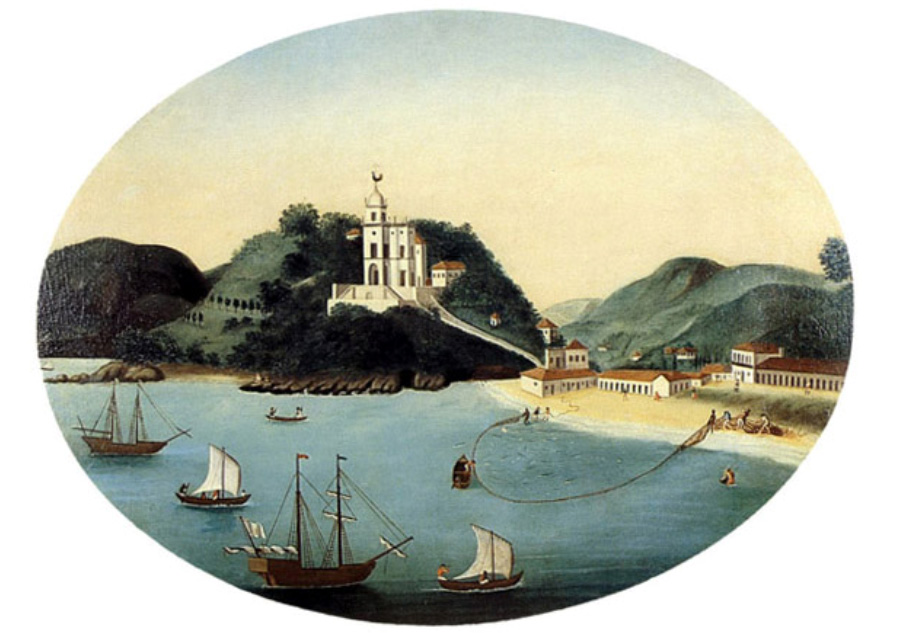
\includegraphics{figures/LeandroJoaquim-Gloria.jpg}
\caption{Leandro Joaquim (1738--1798). Igreja e Praia da Glória,
1790}\label{fig:joaquim}
}
\end{figure}

A série combina cenas oficiais de acontecimentos militares, ambientadas
no centro da cidade ou em seu porto, com representações, à primeira
vista anódinas, dos arredores da cidade. Não obstante a variedade de
cenas, a encomenda unitária sinaliza a intenção de formar uma imagem
global da sede administrativa do vice-reino para consumo interno. Assim,
distingue-se dos mapas e perfis urbanos produzidos para uso da Coroa
enquanto instrumentos de dominação, como os panoramas coetâneos de
Carlos Julião (1740--1811) e Luís dos Santos Vilhena (1744--1814),
aproximando-se do conjunto pictórico produzido pelos artistas franceses
a mando de D. João VI a partir de 1816. A chamada ``Missão artística
francesa'', vista desde Gonzaga Duque
\autocite[p.~257]{gonzagaduque:1995arte} até Bosi
\autocite[p.~228]{bosi:2011cultura} como um momento de ruptura com a
tradição colonial para inserção de um componente importado, insere-se,
pelo contrário, mais propriamente na continuidade do emergente cenário
de cultura urbana do Rio de Janeiro já promovido pelos vice-reis do que
se constituiria em inovação conceitual.

Nicolas-Antoine Taunay (1755--1830) e seu filho, Félix-Émile
(1795--1881), especializados em pintura de paisagem, produzem vasto
material iconográfico sobre o município da Corte, tanto em sua área
urbana quanto no entorno. O monumental panorama do Rio de Janeiro,
executado por Nicolas na França em 1824 com base em remessa de estudos
por Félix, tem lugar de honra nesse ciclo imagético cuja função evidente
é exaltar a dignidade da Capital do Reino e do Império perante a um
público europeu pouco afeito a reconhecer a legitimidade de um poder
ultramarino {[}\textcite{pereira:1994romantismo}; barata:1996alguns{]}.

Ressalta-se, por outro lado, a iconografia ``menor'' de Nicolas no Rio
de Janeiro, em particular as duas vistas do Outeiro da Glória. A
primeira composição, executada já em 1816, é visivelmente baseada na
mesma vista de Leandro Joaquim. Evidencia-se o reconhecimento, por parte
do recém-chegado francês, de uma cultura visual local, mais do que a
simples substituição da tradição colonial por um ``formalismo
indiferente à realidade brasileira''
\autocite[p.~49]{campofiorito:1983historia}. A segunda vista da Glória,
pintada em 1824, opera uma saborosa mescla do tema rococó do embarque
mítico, com reminiscências de Watteau, e de uma ênfase na paisagem
natural sobrepujando os elementos arquitetônicos (Figura
\ref{fig:nicolas}). Somente nesta última vista, executada pouco antes do
retorno de Nicolas à França, é que se percebe o início de um
distanciamento com respeito à pintura documental carioca do final do
século XVIII, substituída pelas referências mais diretas à arte europeia
recente.

\begin{figure}
\hypertarget{fig:nicolas}{%
\centering
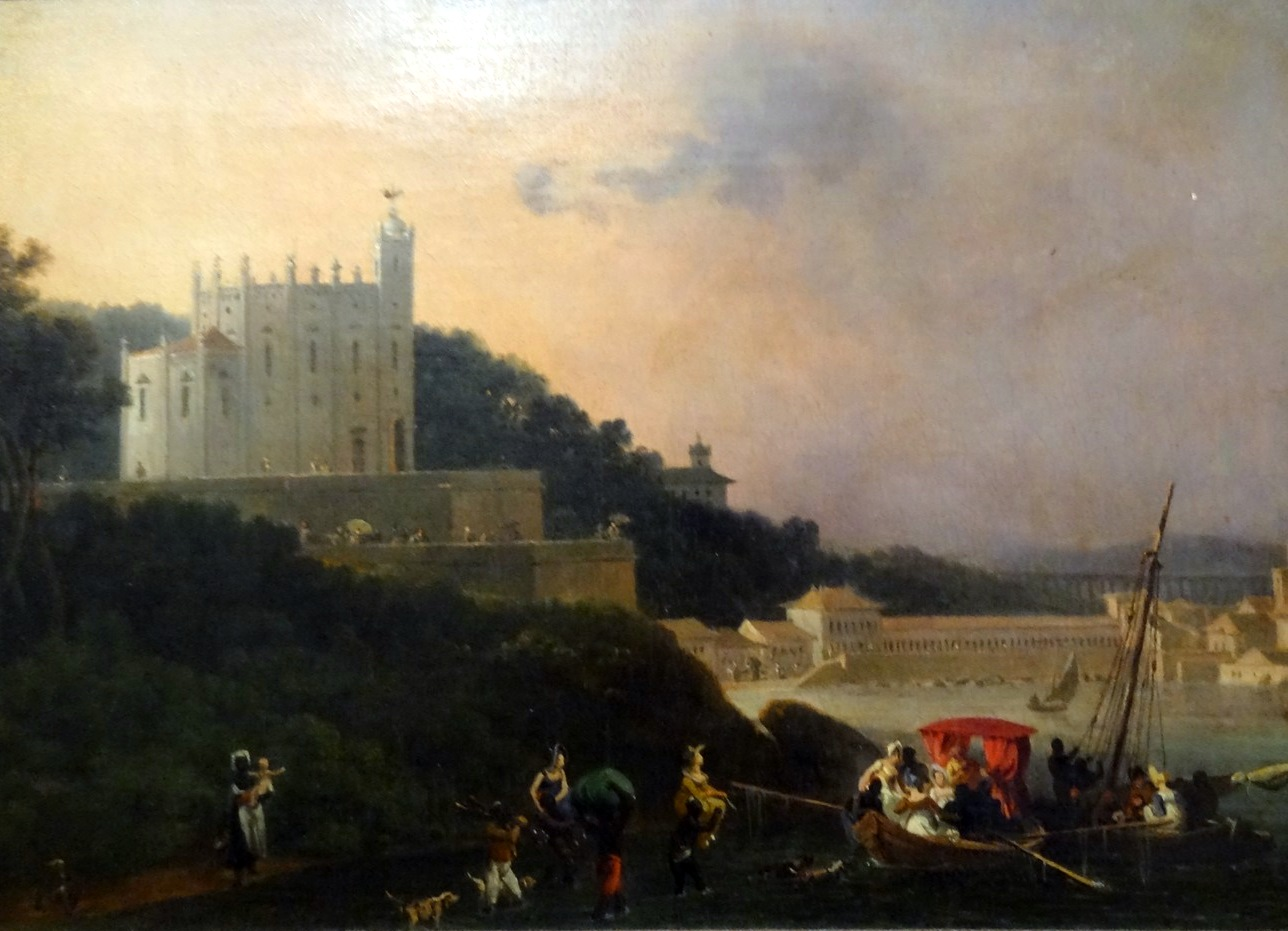
\includegraphics{figures/mar_rio_taunay_gloria_1824.jpeg}
\caption{Nicolas-Antoine Taunay (1755--1830). Glória,
1824}\label{fig:nicolas}
}
\end{figure}

\hypertarget{sublime-natureza-e-cidade}{%
\section{Sublime, Natureza e Cidade}\label{sublime-natureza-e-cidade}}

Debret, pintor de história oficial da corte portuguesa no Brasil, tem
sua produção atualmente mais reconhecida à margem das encomendas
oficiais, por meio da publicação do \emph{Voyage pittoresque et
historique au Brésil} (1834). Sua vista de Taubaté, registrada em
aquarela em 1827, é significativa de uma divergência ainda maior com
respeito à pintura oficial. Apresenta a cidade paulista numa grade
acanhada, não representativa da verdadeira fisionomia da cidade
\autocite{almanaqueurupes:2013arquiteto}, apequenada diante da escala da
paisagem natural (Figura \ref{fig:taubate}). O tema da natureza
sobrepujando a urbanização é, sabidamente, favorecido pelos viajantes
estrangeiros do século XIX, em obras como a célebre representação de
Ouro Preto por Thomas Ender (1817), o panorama de Vila Boa (Goiás) por
William Burchell (1827) ou a vista da Baía de Guanabara por Maria
Graham. É certo que tais imagens, tributárias do conceito de Sublime
oriundo do Romantismo europeu, sinalizam um espírito de exotismo
modelado no discurso iluminista de superioridade da natureza cultivada e
beneficiada pelos europeus, propalado pelo naturalista francês, o Conde
de Buffon (1707--1788) \autocite{palazzo:2002mitos}. No entanto, o tipo
figurativo da cidade em meio à natureza extrapola, em meados do século
XIX, o olhar condescendente dos viajantes europeus pela alteridade, para
ser adotado também pelos artistas brasileiros.

\begin{figure}
\hypertarget{fig:taubate}{%
\centering
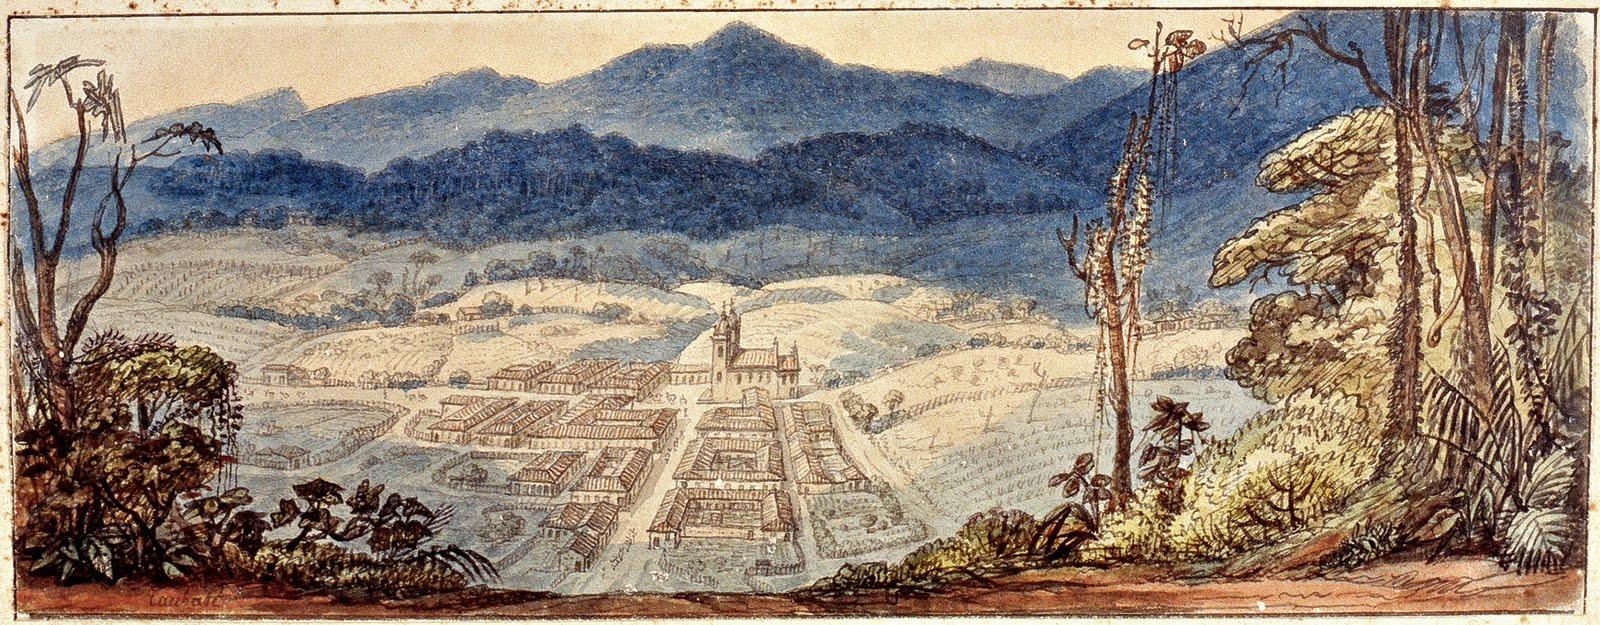
\includegraphics{figures/jb_debret_taubate.jpeg}
\caption{Jean-Baptiste Debret (1768--1848). Vista de Taubaté,
1827}\label{fig:taubate}
}
\end{figure}

Nas exposições gerais de belas artes, realizadas com periodicidade
irregular a partir de 1840, a pintura de paisagem só perde, em
quantidade de obras expostas, para os gêneros mais facilmente executados
do retrato e da natureza morta, mas deixa para trás a pintura histórica
e até mesmo a religiosa \autocite{squeff:2012galeria}. A paisagem do Rio
de Janeiro tomada do alto da Serra de Petrópolis, pintada em 1857 por
Agostinho José da Motta (1824--1878), explicita a fusão entre a pintura
de paisagem e o conceito de vista urbana como tema necessário à
afirmação nacional do Brasil (Figura \ref{fig:motta}). Nessa obra, a
cidade do Rio de Janeiro é apenas discernida pelo perfil de suas
montanhas no horizonte, eliminando-se qualquer indício de civilização em
prol da pujança geológica e florística.

\begin{figure}
\hypertarget{fig:motta}{%
\centering
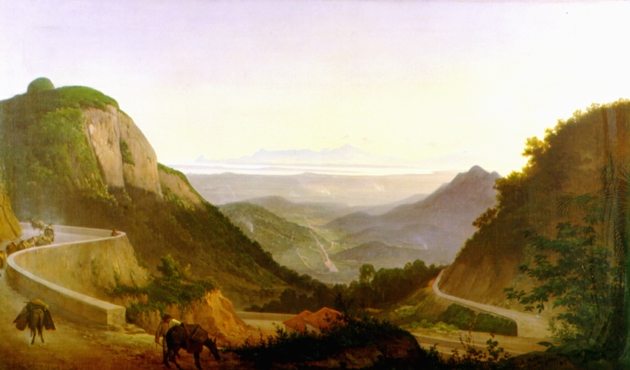
\includegraphics{figures/Agostinho_Jose_da_Mota_-_Paisagem_do_Rio_de_Janeiro.jpg}
\caption{Agostinho José da Motta (1824--1878). Paisagem do Rio de
Janeiro tomada do alto da Serra de Petrópolis, 1857}\label{fig:motta}
}
\end{figure}

Com o crescente mercado de estampas a partir do período regencial e,
mais tarde, de fotografias, a tipologia da vista urbana firma-se como
produto não apenas valorizado na Academia Imperial de Belas Artes
(AIBA), mas igualmente ao gosto do público, consumidor tanto de cenas da
vida cotidiana quanto de paisagens dos arredores da Capital ou das
províncias \autocite[p.~56]{turazzi:2009iconografia}. A produção
pictórica carioca, vinculada à herança deixada pelas obras dos Taunay
retratando a floresta da Tijuca, a lagoa Rodrigo de Freitas e outras
áreas suburbanas do Município da Corte, assume a idiossincrasia de
exaltar a cultura nacional por meio da afirmação de sua própria
insignificância perante a força da natureza.

A Exposição de História do Brasil, realizada no Rio de Janeiro em 1881,
não alinha em suas galerias de arte nada além de vistas da Capital, as
quais se distribuem entre o panorama urbano documental e as cenas da
pujante natureza e relevo entre os quais a própria cidade se perde. O
próprio \emph{Mappa architectural do Rio de Janeiro,} desenhado por João
da Rocha Fragoso e litografado em 1874, oferece, em vez da exuberante
natureza, cândida visão da Capital com seu tecido edificado de origem
colonial, patente confissão da pitoresca especificidade brasileira em
contraste com a grandiloquência das capitais europeias.

O prestígio artístico e crítico de Araújo Porto-Alegre alavancado em
prol do Romantismo, e as concomitantes campanhas etnográficas inspiradas
na missão do IBGE de se constituir as bases ideológicas da nação,
contribuem para fortalecer a busca por imagens representativas do
caráter nacional. Durante algum tempo, a iconografia da Guerra do
Paraguai catalisa esse ímpeto simultâneo pelo Sublime e pela glória do
Brasil. Nos últimos anos do Império, porém, recrudesce a insistência na
produção de uma arte pictórica de reconhecível caráter nacional, indo
além da glorificação romântica da natureza e do pitoresco.

A limitada produção pictórica das províncias não adere, num primeiro
momento, a esse movimento crítico de complementação da vista urbana
oficial pela paisagem sublime engolindo a escala da cidade. As vistas da
cidade de Porto Alegre durante a segunda metade do século XIX, assim
como a fotografia de Militão Augusto de Azevedo em São Paulo por volta
de 1860, conformam-se ao modelo da vista documental de caráter oficial
--- confronte-se com a diversidade de perspectivas tomadas pelo
fotógrafo Georges Leuzinger no Rio de Janeiro da mesma época. Mais
marcante ainda é o panorama do Desterro (Figura \ref{fig:desterro},
atual Florianópolis) executado em 1847 pelo jovem Victor Meirelles
(1832--1903), diretamente baseado na vista do Rio de Janeiro desde o
Morro de Santo Antônio, de Nicolas Taunay (1818). Trata-se, portanto, de
uma obra inserida na linhagem da vista urbana documental, recusando-se a
qualquer ruptura com a iconografia mais convencional, bem como,
reciprocamente, a qualquer aproximação com a incipiente tradição da
vista urbana romântica.

\begin{figure}
\hypertarget{fig:desterro}{%
\centering
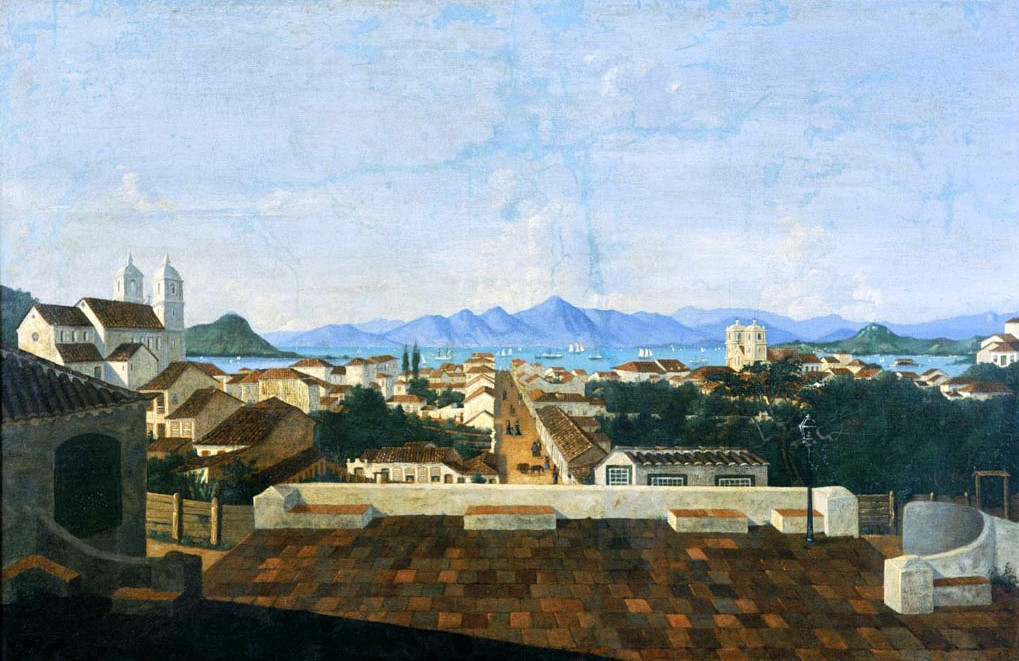
\includegraphics{figures/Victor_Meirelles_-_Vista_do_Desterro_-_c._1847.jpg}
\caption{Victor Meirelles (1832--1903). Panorama do Desterro,
1847}\label{fig:desterro}
}
\end{figure}
